\PassOptionsToPackage{full}{textcomp}
\documentclass[a4paper, twoside, nobib]{tufte-book}
\hypersetup{colorlinks}

%%%%%%%%%%%%%%%%%%%%%%%%%%%%%%%%%%%%%%%%%%%%%%%%%%%%%%%%%%%%%%%%%%%%%%%%%%%%%%%
% metadata

\title{ML-based precision medicine in ischemic heart disease}
\author[Peter Christoffer Holm]{Peter Christoffer Holm}
\publisher{%
    Graduate School of Health and Medical Sciences
    University of Copenhagen%
}

%%%%%%%%%%%%%%%%%%%%%%%%%%%%%%%%%%%%%%%%%%%%%%%%%%%%%%%%%%%%%%%%%%%%%%%%%%%%%%%
% biblatex configuration

\usepackage[%
    style=verbose-note,
    %% disable these fields in the citation %%
    url=false,
    isbn=false,
    doi=false,
    eprint=false,
    eprint=false,
    %%%%%%%%%%%%%%%%%%%%%%%%%%%%%%%%%%%%%%%%%%
    date=year,
    maxcitenames=2,     % when should "et al." be triggered?
    maxbibnames=4,      % when should "et al." be triggered? (in bib)
    sorting=nty,        % name, title, year
    autocite=footnote,  % put citation in sidenotes 
    citereset=chapter,  % reset citation tracker at each chapter
    citetracker=strict,
    trackfloats=true
]{biblatex}

\DeclareCiteCommand{\cite}
  {\usebibmacro{prenote}}
  {\usebibmacro{citeindex}%
   \usebibmacro{footcite}}
  {\multicitedelim}
  {\usebibmacro{cite:postnote}}

\newcommand{\sidecite}[2][0em]{%
	\unskip\sidenote[][#1]{\cite{#2}}%
}

\renewbibmacro{in:}{}
\AtEveryCitekey{%
    \clearfield{pagetotal}%
    \clearfield{eprint}%
    \clearfield{url}%
    \clearfield{pages}%
    \clearfield{series}%
    \clearfield{volume}%
    \clearfield{number}%
    \clearfield{issue}%
    \clearlist{location}%
    \clearname{editor}%
}
\addbibresource{assets/pch-thesis.bib}

% fix appearance of cited preprints
\DeclareSourcemap{
    \maps[datatype=bibtex]{
        \map{
            \pertype{online}
            \step[typesource=online, typetarget=article]
            \step[fieldsource=eprinttype, fieldtarget=journaltitle]
            \step[fieldsource=journaltitle,
                match={arxiv}, replace={arXiv}]
        }
    }
}

\DeclareStyleSourcemap{
    \maps[datatype=bibtex]{
        \map{
            \pertype{inproceedings}
            \step[fieldset=publisher, null=true]
        }
    }
}

%%%%%%%%%%%%%%%%%%%%%%%%%%%%%%%%%%%%%%%%%%%%%%%%%%%%%%%%%%%%%%%%%%%%%%%%%%%%%%%
% load packages

% fonts
\usepackage[T1]{fontenc}

\usepackage[p, osf]{ETbb}  % osf in text, tabular lining figures in math
\usepackage[scaled=.95,type1]{cabin}  % sans serif in style of Gill Sans
\usepackage[libertine, vvarbb]{newtxmath}

% misc
\usepackage{amsmath}
\usepackage{amsfonts}
\usepackage{microtype}
\usepackage{booktabs}
\usepackage{tabularx}
\usepackage{multicol}
\usepackage{makecell}
\usepackage{pdfpages}
\usepackage{appendix}
\usepackage{siunitx}
\usepackage{todonotes}

\usepackage{subcaption}
\captionsetup{font=footnotesize}    

\usepackage{marginfix}
\usepackage{appendix}
\usepackage{twemojis}
\usepackage{cleveref}
\usepackage{pgffor}
\usepackage{relsize}  % easy scaling of fonts
\usepackage{bm}

%%%%%%%%%%%%%%%%%%%%%%%%%%%%%%%%%%%%%%%%%%%%%%%%%%%%%%%%%%%%%%%%%%%%%%%%%%%%%%%

%\newcommand{\mbf}[1]{\bm{\mathrm{#1}}}
\DeclareMathOperator{\EX}{\mathbb{E}} % expected value
\DeclareMathOperator{\PR}{\Pr} % probability 
\DeclareMathOperator{\I}{\mathbb{1}}  % indicator 
\DeclareMathOperator{\CIF}{CIF}
\DeclareMathOperator{\card}{\raisebox{-.22ex}{\#}}

\newcommand{\mat}[1]{\bm{\mathsf{#1}}}
\renewcommand{\vec}[1]{\bm{#1}}

\newcommand{\giv}{\,|\,}
\newcommand{\lik}{\mathscr{l}}
\newcommand{\Lik}{\mathcal{L}}


\newcommand{\Tic}{{T_{\mathrm{c}}}}
\newcommand{\Tid}{{T_{\mathrm{d}}}}
\newcommand{\Cid}{{C_{\mathrm{d}}}}

\newcommand{\tic}{t}
\newcommand{\tid}{\tau}

\DeclareMathOperator*{\argmin}{arg\,min}
\newcommand{\diff}{\mathrm{d}}

\newcommand{\xa}{\mathbf{x}}
\newcommand{\xb}{\check{\xa}}
\newcommand{\hzt}{\lambda_0\mspace{-1mu}(t)}

%%%%%%%%%%%%%%%%%%%%%%%%%%%%%%%%%%%%%%%%%%%%%%%%%%%%%%%%%%%%%%%%%%%%%%%%%%%%%%%

% enumerate
\usepackage[inline]{enumitem}
\renewlist{enumerate*}{enumerate*}{1}
\setlist[enumerate*]{
    label=(\roman*), itemjoin={{; }}, itemjoin*={{; and }}
}

% context aware quotation marks
\usepackage{csquotes}  
\renewcommand{\mkcitation}[1]{~\autocite{#1}}

% acro 
\usepackage[nohyperlinks]{acronym}
%\renewcommand*{\acsfont}[1]{{\relsize{+0.5}\smallcaps{#1}}}

% tikz 
\usepackage{tikz}
\usepackage{pgfplots}
\usepgfplotslibrary{groupplots}
\usepackage{listofitems}
\usepackage{contour}
% \usetikzlibrary{external}
% \tikzexternalize[optimize=false, prefix=figures/]

\usetikzlibrary{positioning}
\usetikzlibrary{arrows,shapes}
\usetikzlibrary{arrows.meta} 
\usetikzlibrary{graphs} 
\usetikzlibrary{quotes} 
\usetikzlibrary{decorations.text}
\usetikzlibrary{decorations.markings}
\usepackage{annotate-equations}

\definecolor{color0}{HTML}{001118}
\definecolor{color1}{HTML}{005e72}
\definecolor{color2}{HTML}{0a9395}
\definecolor{color3}{HTML}{93d1bc}
\definecolor{color4}{HTML}{e8d8a5}
\definecolor{color5}{HTML}{ed9a00}
\definecolor{color6}{HTML}{ca6702}
\definecolor{color7}{HTML}{ba3d02}
\definecolor{color8}{HTML}{ae1f11}
\definecolor{color9}{HTML}{9a2126}

% for graphics / images
\usepackage{graphicx}
\setkeys{Gin}{width=\linewidth,totalheight=\textheight,keepaspectratio}
\graphicspath{{graphics/}}

% adjust verbatim environments
\usepackage{fancyvrb}
\fvset{fontsize=\normalsize}

%%%%%%%%%%%%%%%%%%%%%%%%%%%%%%%%%%%%%%%%%%%%%%%%%%%%%%%%%%%%%%%%%%%%%%%%%%%%%%%
% custom macros

% Hanging parentheses and asterisks
\newcommand{\hangp}[1]{\makebox[0pt][r]{(}#1\makebox[0pt][l]{)}}
\newcommand{\hangstar}{\makebox[0pt][l]{*}}

% prints the month name (e.g., january) and the year (e.g., 2008)
\newcommand{\monthyear}{%
  \ifcase\month\or January\or February\or March\or April\or May\or June\or
  July\or August\or September\or October\or November\or
  December\fi\space\number\year
}

% misc
\newcommand{\na}{\quad--}
\newcommand{\blankpage}{\newpage\hbox{}\thispagestyle{empty}\newpage}

%%%%%%%%%%%%%%%%%%%%%%%%%%%%%%%%%%%%%%%%%%%%%%%%%%%%%%%%%%%%%%%%%%%%%%%%%%%%%%%
\begin{document}

\frontmatter
\maketitle

\begin{@empty}
~\vfill
\thispagestyle{empty}
\setlength{\parindent}{0pt}
\setlength{\parskip}{\baselineskip}

\smallcaps{Candidate}

\textbf{Peter Christoffer Holm}, MSc

Novo Nordisk Foundation Center for Protein Research,
University of Copenhagen, Denmark

\smallcaps{Supervisors}

\textbf{Søren Brunak}, PhD, Professor 
(principal supervisor)

Novo Nordisk Foundation Center for Protein Research, 
University of Copenhagen, Denmark

\textbf{Henning Bundgaard}, PhD, Dr.Med, Professor 
(co-supervisor)

Department of Cardiology,
Copenhagen University Hospital, Denmark

\textbf{Karina Banasik}, PhD, Associate Professor 
(co-supervisor)

Novo Nordisk Foundation Center for Protein Research, 
University of Copenhagen, Denmark

\vspace{2em}

\par\smallcaps{Published by the \thanklesspublisher}

\vspace{5em}

\par This document was created using the \LaTeX{} typesetting software.
The layout is based on the \texttt{tufte-latex} document class,
and the main body of the text is set in \textsf{ETbb} and \textsf{Libertine}.
Unless otherwise indicated, all figures and graphics in the main text
are either the property of the author or are in the public domain.

%\par\textit{First printed, \monthyear}

Copyright \copyright\ \the\year\ \thanklessauthor
\end{@empty}
      % [ ]
\begin{@empty}
\thispagestyle{empty}
\setlength{\parindent}{0pt}
\setlength{\parskip}{\baselineskip}

\chapter*{Preface}

This PhD thesis has been submitted
to the Graduate School of Health and Medical Sciences,
University of Copenhagen.

The work presented in this thesis was performed
at the Novo Nordisk Foundation Center for Protein Research (CPR),
University of Copenhagen, Denmark.

I declare no conflicts of interests.

\begin{flushright}
    Copenhagen, December 2023 \\
    Peter Christoffer Holm
\end{flushright}
\end{@empty}
        % [ ]

\cleardoublepage
\tableofcontents
\listoffigures
\listoftables

\chapter*{List of Acronyms}
\begin{acronym}[NSTEMI]
\acro{IHD}{ischemic heart disease}
\acro{MI}{myocardial infarction}
\acro{UA}{unstable angina}
\acro{ECG}{electrocardiogram}
\acro{NSTEMI}{non-ST-elevation myocardial infarction}
\acro{STEMI}{ST-elevation myocardial infarction}
\acro{CABG}{coronary artery bypass grafting}
\acro{PCI}{percutaneous coronary intervention}
\acro{CI}{confidence interval}
\acro{OR}{odds ratio}
\acro{PK}{pharmacokinetics}
\acro{SNP}{single-nucleotide polymorphism}
\acro{EHR}{electronic health record}
\acro{ML}{machine learning}
\acro{AI}{artificial intelligence}
\acro{DL}{deep learning}
\acro{SGD}{stochastic gradient descent}
\acro{ReLU}{rectified linear unit}
\acro{tanh}{hyperbolic tangent}
\acro{HPO}{hyperparameter optimization}
\acro{SHAP}{Shapley additive explanations}
\acro{XAI}{explainable artificial intelligence}
\acro{MACE}{major adverse cardiovascular event}
\acro{CIF}{cumulative incidence function}
\acro{CDF}{cumulative distribution function}
\acro{PDF}{cumulative probability function}
\acro{CHF}{cumulative hazard function}
\end{acronym}
        % [ ]
\chapter{List of Manuscripts}
\section{Manuscripts included in this thesis}
\subsection{Paper 1}

Amalie D. Haue*, 
\underline{Peter C. Holm}*, 
\marginnote{%
  An asterisk (*) denotes equal contribution.

  \noindent
  This manuscript was also included in the thesis of Amalie D. Haue.
}
Karina Banasik, Agnete T. Lundgaard, Victorine P. Muse, Timo Röder, 
David Westergaard, Piotr J. Chmura, Alex H. Christensen, Peter E. Weeke, 
Erik Sørensen, Ole B. V. Pedersen, Sisse R. Ostrowski, Kasper K. Iversen, 
Lars V.  Køber, Henrik Ullum, Henning Bundgaard, 
and Søren Brunak:
\textbf{\enquote{%
    Subgrouping multimorbid patients with ischemic heart disease 
    by means of unsupervised clustering: 
    A cohort study of 72,249 patients 
    defined comprehensively by diagnoses prior to presentation
}}.
\textit{%
    Submitted for publication (under review).
    Preprint posted on medRxiv (2023): 2023-03.
}

\subsection{Paper 2}
\underline{Peter C. Holm},
\marginnote{%
  An ealier version of this  manuscript was included in the thesis of 
  Amalie D. Haue.%
}
Amalie D. Haue,  
David Westergaard, Timo Röder, Karina Banasik, Vinicius Tragante, 
Alex H. Christensen,  Laurent Thomas,  Therese H. Nøst, Anne-Heidi Skogholt, 
Kasper K. Iversen, Frants Pedersen, Dan E. Høfsten, Ole B. Pedersen,  
Sisse Rye Ostrowski, Henrik Ullum, Mette N. Svendsen, Iben M. Gjødsbøl, 
Thorarinn Gudnason, Daníel F. Guðbjartsson,  Anna Helgadottir, Kristian Hveem,  
Lars V. Køber,  Hilma Holm, Kari Stefansson,  Søren Brunak,  
and Henning Bundgaard:
\textbf{\enquote{%
    Development and validation of a neural network-based survival model 
    for mortality in ischemic heart disease%
}}.
\textit{%
    Submitted for publication (under review).
    Preprint posted on medRxiv (2023): 2023-06.
}

\subsection{Paper 3}
\underline{Peter C. Holm},
\todo{add more authors once manuscript is ready}
\ldots, Henning Bundgaard, and Søren Brunak
\enquote{%
    Development of a neural network-based competing risk model 
    for individualized prognostication in ischemic heart disease 
    using a large database of electronic health records 
    and clinical registries}
preprint: \textit{medRxiv (2023): 2023-12.}

\clearpage
\section{Manuscripts not included in this thesis}

\subsection{Paper 4}
Isa K. Kirk, \ldots, 
\underline{Peter C. Holm},
\ldots, Søren Brunak
\textbf{\enquote{%
    Linking glycemic dysregulation in diabetes to symptoms, 
    comorbidities, and genetics through EHR data mining
}}
in \textit{eLife} (2019)

\subsection{Paper 5}
Ina H. Laursen, \ldots, 
\underline{Peter C. Holm},
\ldots, Henrik Ullum
\textbf{\enquote{%
    Cohort profile: Copenhagen Hospital Biobank - Cardiovascular Disease Cohort
    (CHB-CVDC): Construction of a large-scale genetic cohort to facilitate a
    better understanding of heart diseases
}}
in \textit{BMJ Open} (2021)

\subsection{Paper 6}
Amalie D. Haue, \ldots, 
\underline{Peter C. Holm},
\ldots, Henning Bundgaard, and Søren Brunak
\textbf{\enquote{%
    Temporal patterns of multi-morbidity in 
    570157 ischemic heart disease patients: 
    a nationwide cohort study
}}
in \textit{Cardiovascular Diabetology} (2022)

\subsection{Paper 7}
Alex W. Jung, 
\underline{Peter C. Holm}, \ldots, 
Søren Brunak, and 
Moritz Gerstung
\textbf{\enquote{%
    Multi-cancer risk stratification based on national health data: a
    retrospective modelling and validation study
}}
preprint in \textit{medRxiv} (2022)

\subsection{Paper 8}
Karina Banasik, \ldots, 
\underline{Peter C. Holm}, \ldots, 
Thomas F. Hansen
\textbf{\enquote{%
    DanMAC5: a browser of aggregated sequence variants from 8,671 whole genome
    sequenced Danish individuals
}}
in \textit{BMC Genomic Data} (2023)

\subsection{Paper 9}
David Westergaard, \ldots, 
\underline{Peter C. Holm}, \ldots, 
Søren Brunak, and 
Henriette S. Nielsen
\textbf{\enquote{%
    Immune Changes in Pregnancy: Associations with Pre-existing Conditions and
    Obstetrical Complications at the 20th Gestational Week-A Prospective Cohort
    Study
}}
preprint in \textit{medRxiv} (2023)

     % [ ]
\chapter{Summary}
         % [ ]

\cleardoublepage
\chapter{Overview and Structure} \label{intro}

Precision medicine

The primary objective of this thesis is to contribute to the advancement of
precision medicine in the field of ischemic heart disease, with a particular
emphasis on secondary prevention. The research focuses on two main areas: 1)
characterizing multimorbidity in ischemic heart disease and its impact on
disease risk and progression, and 2) developing risk-prediction tools capable
of leveraging heterogeneous healthcare data. For the latter, we have employed
neural network-based survival models designed to accurately handle censored
data.

This thesis investigates how data-driven approaches can enhance the evolution
of precision medicine specifically for ischemic heart disease. While the
research is concentrated on ischemic heart disease and cardiology, the
methodologies and findings could potentially be extrapolated to other medical
fields, given their broad applicability.

The intersection of precision medicine and artificial intelligence represents a
significant paradigm shift, offering the potential to revolutionize how we
diagnose, manage, and treat diseases.

\section{My Thesis}

The overall goal of this dissertation is to present 
our research on the topic of machine-learning based 
precision medicine in ischemic heart disease.
The thesis is written in the form a synopsis 
and is as such based on three key manuscripts around 
which the content of thesis is centered around.

\section{Organization}

\begin{itemize} 

    \item In the chapter \nameref{pm-in-ihd}, I provide an
        in-depth discussion of the pathophysiology and disease manifestations of
        ischemic heart disease, which serves as the focal point of this thesis.
        I offer an overview of the methodologies involved in developing data-driven
        precision medicine. Throughout the thesis, precision medicine is
        primarily contextualized within the frameworks of \enquote{big data} 
        and \enquote{machine learning}.

    \item The chapter \nameref{ml-fundamentals} introduces the core concepts of
        machine learning, with a specific focus on neural networks. While the
        chapter is generally broad in scope, it places particular emphasis on
        the tools and techniques utilized in the research presented.

    \item The final background chapter, \nameref{survival-analysis}, provides a
        comprehensive overview of survival analysis. It further delves into the
        specific approach we have employed for modeling time-to-event data
        using neural networks.  

    \item In \nameref{results}, I summarize each of the three included papers,
        briefly outline the methodologies employed, and highlight the key
        findings.  Additionally, I contextualize the research within the
        broader scientific literature.

    \item In \nameref{conclusions}, I offer final thoughts on the thesis and
        outline areas that warrant further investigation.

    \item The \nameref{appendix} includes the three full-length scientific
        manuscripts that form the core of this thesis.

\end{itemize}

\todo[inline]{Refactor \enquote{Thesis Overview} section.}
           % [ ]

\mainmatter %%%%%%%%%%%%%%%%%%%%%%%%%%%%%%%%%%%%%%%%%%%%%%%%%%%%%%%%%%%%%%%%%%%

\part{Background and Methods}
\chapter{Thesis Objectives and Overview} \label{intro}

The overall aim of this thesis is ...


\vskip 10em

With the advent of large language models (LLMs) like ChatGPT
%------------------------------------------------------------------------------
\marginnote{%
    \textsf{hype}, (noun). [clipping of hyperbole].

    (marketing) promotion or propaganda; especially exaggerated claims. 
    \rightline{\textit{wiktionary.org}}%
}
%------------------------------------------------------------------------------
and text-to-image models such as DALL-E and Midjourney,
there has been a surge of interest in the broader domains of
artificial intelligence and machine-learning.
%
ChatGPT, in particular, stands out as prominent example---%
an LLM-based chatbot developed by OpenAI, 
have managed to impress both the general public aswell 
as researchers across various disciplines.
It has been shown that ChatGPT can pass exams
such as USMLE\footnotemark
~\autocite{openaiGPT42023}

%------------------------------------------------------------------------------
\footnote{%
The United States Medical Licensing Examination (USMLE) 
is a three-step examination program for obtaining a medical license
in the United States of America.
}
%------------------------------------------------------------------------------






It has been claimed that 




However, 




The convergence of precision medicine and artificial intelligence 
stands as a monumental paradigm shift, promising to redefine
the way we diagnose, treat, and manage disease.



It is this author's opinion, 
that the main cause of \enquote{success} of the abovementioned
AI-applications is the combined value of 
absolutelive massive datasets and massive computing power.

This thesis has little to do with the likes of ChatGPT, 
but 

In this thesis, I explore how data-drive approaches
can further the development of precision medicine in ischemic heart disease.

The thesis is structured as follows:
in the chapter \nameref{precision-medicine} I will be introducing the 
concept of precision medicine framed in the context of \enquote{big data}
and \enquote{machine learning}.

In \nameref{ml-fundamentals}

In \nameref{survival-analysis}

In \nameref{results}

In \nameref{conclusions}




Although we in the three manuscripts that forms this thesis 
primarily place a focus on cardiology,
and specifically ischemic heart disease,
the presented methods can be used across many fields of medicine.



       % [X]
\chapter{Machine Learning}

The promise of AI lies in the ability 
to integrate large amounts of data from huge data sets
and almost instantaneously register patterns
with clinical importance.

Machine Learning seeks to let computers learn from data
without them being explicitly programmed.


The Turing test, proposed by Alan Turing in 1950,
tries to answer the question \enquote{can a machine think?}.
A computer passes the test if a human interogator,
after posing a series of written questions,
cannot determine if the responses come from a human or a computer.


\textquote[\autocite{russellArtificial2009}]{%
The quest for \enquote{artificial flight} succeeded 
when engineers and inventors stopped imitating birds 
and started using wind tunnels and learning about aerodynamics.
Aeronautical engineering texts 
do not define the goal of their field as making 
\enquote{machines that fly so exactly like pigeons 
that they can fool other pigeons.}\,}

If the output is a finite set of values
the learning problem is called \textbf{classification},
and if it is a number, then it is called \textbf{regresion}.

In supervised learning, the model observes input-output pairs
and tries to learn a function that maps inputs to outputs.

In unsupervised learning, the model learns patterns in unlabeled input data.

With many machine-learning models, there is a bias--variance tradeoff:
on one end of the spectrum we have simple low-variance models 
such as linear or logistic regression
and on the other end, we have high-variance models
such as neural networks or random forests.

We can estimate the error rate of model
by evaluating it on a test set.
If we are only creating a single model,
then this approach suffices. 
However, we might want to compare many different models,
or slightly tweak an already existing model,
such that we can select the performing version.
If we select the final model based on the test set,
we might inadvertently have biased the process,
and could, in a sense, have overfitted to the test data.
To avoid this, we need to completely hide away the test data
until we are done with training, experimenting, 
and hyperparameter optimization.
To allow this, we instead need three sets of data:

\begin{itemize}
    \item a training set to train or develop candidate models
    \item a validation set to evaluate the candidate models
        and select the best one
    \item a test set do the final unbiased evaluation of model performance
\end{itemize}

Another alternative is using the technique \textit{k}-fold cross-validation.

A model is interpretable if we can inspect the model
and understand why it gave a certain output for a particular input.
An explainable model is one that can help us understand 
why a certain output was produced for a specific input.
Interpretability comes from inspecting the actual model.
Explainability can come from an external process.

Typically there is a distinction between model-based explanations
and post hoc explanations\autocite{vanderveldenExplainable2022}.
The scope of an explanation is the difference between
explanations for a complete model and
explanations for a single output.
Global explanation covers feature importance estimates 
for the entire dataset.
Local explanations, on the other hand, seeks to explain
the impact of the specific example under scrutiny.
A SHAP-waterfall plot is an example of a local explanation.
A saliency map of a chest radiograph that shows
which pixels contributed to the label \enquote{liver cancer}
is another example.

Shapley values measures the marginal contribution
of each individual feature.

One limitation of XAI models is the accuracy and relevance of explanations.
Explainability algorithms such as SHAP are only approximations
of the complete model.
In other words, the fidelity is not perfect and therefore neither
is the explanation.
However, for black-box models such as neural networks,
it is the next best thing.

\section{Neural Networks}

\begin{marginfigure}%
	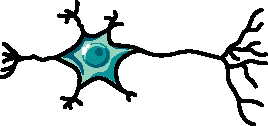
\includegraphics[width=\linewidth]{graphics/neuron}
    \caption[Schematic diagram of a neuron]{%
        Schematic diagram of a neuron.
        A typical neuron has a dendrites, a cell body, and a single axon; 
        the dendrites receive input signals from other neurons,
        and propagates output signals along the axon.
    }
    \label{fig:neuron}
\end{marginfigure}

\begin{marginfigure}%
	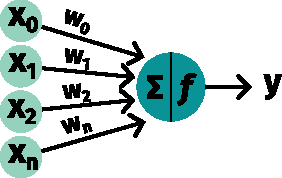
\includegraphics[width=\linewidth]{graphics/perceptron}
	\caption{Schematic diagram of a perceptron}
    \label{fig:perceptron}
\end{marginfigure}

%%%%%%%%%%%%%%%%%%%%%%%%%%%%%%%%%%%%%%%%%%%%%%%%%%%%%%%%%%%%%%%%%%%%%%%%%%%%%%%

Neural networks have been designed
using the archicteture of neurons in a human brain as inspiration.
The simplest model is that of a perceptron, 
which can be seen as a computational approximation
of a real neuron or nerve cell%
\autocite{charniakIntroduction2019}.
A typical neuron has many dendrites, a cell body, and a single axon 
(Figure~\ref{fig:neuron}).
The dendrites carries the input signal to a neuron,
and if the cumulative signal is great enough%
\sidenote{
    This threshold is known as 
    the \textit{threshold potential},
    and is typically between -50 and -55 mV.
}, 
then the neuron will propagate an action potential down the axon%
\autocite{seifterConcepts2005}.
In similar fashion, a perceptron receives may receive many different inputs
and produces a single output (Figure~\ref{fig:perceptron}).
In the case of a neuron, the \enquote{all-or-none} principle means
that nerve cells either signals at full strength or not all.
For a perceptron, this priniciple can be emulated
with the followingly step function:

\begin{equation}
    f_{\phi}(\mathbf{x})  = 
        \begin{cases}
            1 & \text{if } b + \mathbf{w} \cdot \mathbf{x} > 0\\
            0 & \text{otherwise}
        \end{cases}
\end{equation}

By combing many thousands of such neurons,
in a multilayer-perceptron or artificial neural network,
we can create a model that, 
can learn even the most complex of patterns.
Deep learning is at its core a form of representation learning.
Each layer in a neural network is a different representation,
and by stacking several of such layers on top of each others,
the representation in one hidden layer
feeds into the next layer and
is thereby being transformed into an even more abstract representation%
\autocite{estevaGuide2019}.

%%%%%%%%%%%%%%%%%%%%%%%%%%%%%%%%%%%%%%%%%%%%%%%%%%%%%%%%%%%%%%%%%%%%%%%%%%%%%%%
% insert example of abstract representations in a computervis model
%%%%%%%%%%%%%%%%%%%%%%%%%%%%%%%%%%%%%%%%%%%%%%%%%%%%%%%%%%%%%%%%%%%%%%%%%%%%%%%


\section{Regularization}

One approach to avoid overfitting in neural networks
is a technique known as dropout.
At each step of model training,
a random set of nodes in the network are disabled.
In a sense, the result is a rough approximation of 
an ensemble of different networks.


Dropout introduces noise during training
and thereby forces the network to be less senstive of noise.
Hidden units trained with dropout needs to be useful 
with or without the presence of neighboring units.

%%%%%%%%%%%%%%%%%%%%%%%%%%%%%%%%%%%%%%%%%%%%%%%%%%%%%%%%%%%%%%%%%%%%%%%%%%%%%%%

\section{Miscellaneous}

In his review on artificial intelligence in medicine%
\autocite{topolHighperformance2019}, 
Eric Topol expresses his view that in the future
\blockquote{%
almost every type of clinician, ranging from specialty doctor to paramedic,
will be using AI technology, and in particular deep learning [...]
}.

The ability to predict adverse outcomes could make  
healthcare resources more efficient.

Systematic deugging and continuous monitoring and validation 
is of utmost importance if we are to release AI algorithms into the wild%
\autocite{topolHighperformance2019}.

There has been much discussion about, and there are many opinions on, 
the black-box nature of many machine learning algorithms and 
how it should or should not affect the clinical use of such 
\autocite{topolHighperformance2019, gunningXAI2019, vanderveldenExplainable2022}.


In computer vision tasks in the medical domain,
deep-learning models have achieved physician-level performance
in many different diagnostic tasks
ranging from \todo{finish sentence}.
   % [X]
\chapter{Time-to-Event Prediction with Neural Networks}
\label{survival-analysis}

% marginnote {{{
\marginnote{%
    \setlength{\parindent}{0pt}
    \vskip 1em
    What is survival analysis?
    \begin{description}[leftmargin=!, labelwidth=3em]
        \item[outcome] time until an event occurs.
            Can be measured in seconds, days, months, etc.
        \item[event] death, relapse, remission, engine failure, etc.
    \end{description}
    
    \begin{center}
    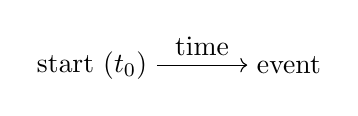
\begin{tikzpicture}
        \noindent
        \node (a) at (2.5, 0) {event};
        \node (b) at (0, 0) {start (\(t_0\))} edge ["time", ->] (a);
    \end{tikzpicture}
    \end{center}
}
% }}}

In the previous chapter, 
I gave an overview of machine learning and neural networks,
highlighting key ideas and concepts related to the studies in this thesis.
Neural networks specifically, 
were used in \studyii{} and \studyiii{} to develop
prediction models for ischemic heart disease.
These models, however, diverge from classical neural network methods.
Instead, they include modifications that make them applicable
in modelling and analysis of time-to-event data.
This chapter will provide an introduction to the fundamentals
of survival analysis and will cover the
theory that enables the implementation of such analyses with
neural network models.
% The chapter concludes with a discussion on different 
% validation methods for time-to-event prediction models.

\section{What is Survival Analysis?}

Generally, 
survival analysis is the collection of statistical methods
for the modelling and analysis of time-to-event data,
which is data where the outcome variable of interest 
is the time until \enquote{something} happens.~%
~\autocite{kleinbaumSurvival2011}
This \enquote{something} is a particular event of interest,
which, depending on the type of analytical problem, 
could be cancer relapse, 
diabetes remission,
or death.
In cardiovascular research, 
common examples of time-to-event outcomes include
\begin{enumerate*}
    \item time to death due to any cause (all-cause mortality)
    \item time to death due to a specific cause,
        e.g. sudden cardiac arrest
    \item time to first occurence of a \ac{MACE}
\end{enumerate*}.
To figure out what processes and characteristics 
that are associated with such events, 
in survival analysis, we try to model the relationship between
explanatory variables and the number of weeks, months, or years 
until that particular event is likely to occur. 

% marginnote{{{
\marginnote{%
    Survival analysis have applications outside biomedical research.
    In engineering, it is called \textit{reliability analysis} and
    is used to model the time-to-failure of system-critical components 
    such as e.g. bearings or valves.
}% }}}

Although this task can be daunting in its own right, 
an additional complication to survival analysis 
is the presence of observations that are subject to 
censoring.
This concept, censoring, refers to cases 
where the event of interest has not been observed 
before the end of follow-up, 
e.g. when a study or experiment has to be stopped.
In such cases, 
we would know that a given subject did not experience a relapse 
in the three months he or she was included in the study, 
but after the study period ends, 
we have no information on the status of the patient. 
Including and utilizing this partial information
is a cornerstone in many survival analysis problems.

There exists different forms of censoring,
such as right censoring, left censoring, and interval censoring.
In the study designs used throughout this thesis 
we have only had to deal with right censoring,
the most common form of censoring,
so the two other types will not be described further.
See instead the text book by \citeauthor{kleinSurvival2003} 
for more details on this.
~\autocite{kleinSurvival2003}

\section{Fundamentals of Survival Analysis}

In survival analysis, 
the central outcome variable is survival time,
a non-negative random variable denoted as \(T\). 
When refering to specific values of \(T\), 
a lower case \(t\) is typically used.  
A survival dataset \(\mathfrak{D}\) of size \(N\) is given by
\begin{equation}
    \mathfrak{D}_N = \{(t_i, \sigma_i, \vec{x}_i) \mid i = 1, \ldots, N\} 
\end{equation}
where \(t_i = \min(T_{i}, C_i) \) is the survival time 
for the \(i\)th subject,
with \(T_i\) denoting the survival time
and \(C_i\) denoting the censoring time. 
Also, \(\vec{x}_i = (x_1, x_2, \dots, x_p)'\) is the covariate vector
and \(\sigma_i\) is the event indicator, which is defined as
\begin{equation}
    \label{eq:sigma-def}
    \sigma_i =
        \begin{cases}
            0 & \text{if subject is censored} \; (T_i >    C_i) \\
            1 & \text{if event is observed} \; (T_i \leq C_i)
        \end{cases}
\end{equation}

In the following, I will initially be assuming that \(T\) is 
continuous and that there is an absence of competing risks, 
however both of these assumptions will later be relaxed in the discussion 
of competing risks and discrete-time survival analysis.

\subsection{Basic Survival Quantities}
\label{sub:survival-quantities}

% figure: theoretical survival function{{{
\begin{marginfigure}%
	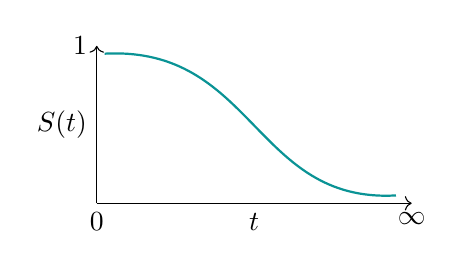
\begin{tikzpicture}[scale=2]
	  \draw[->] (0, 0) --  (2,0) 
		node[pos=0.0, below] {$0$}
		node[pos=0.5, below] {$t$}
		node[pos=1.0, below] {$\infty$};
	  \draw[->] (0, 0) --  (0,1) 
		node[pos=1.0, left] {$1$}
		node[pos=0.5, left] {$S(t)$};
	  \draw[-, color=color2, thick] 
		(0.05, 0.95) .. controls (1, 1) and (1, 0) .. (1.90, 0.05);
	\end{tikzpicture}
    \caption[A Theoretical Survival Function]}}

In survival analysis, 
the central function of interest is 
the survival function \(S(t)\), 
that represents the probability 
of an individual still being alive after 
some specified duration of time, we have that 
%
\begin{equation}
    S(t) = \PR (T > t), \quad 0 < t < \infty.
\end{equation}

The survival function is 
the integral of the probability density function, \(f(t)\),
and is the complement to the cumulative distribution function, \(F(t)\),
which means that
~\autocite{kleinSurvival2003}
%
\begin{equation}
    S(t) = 1 - F(t) 
    \quad \text{and} \quad 
    S(t) = \int_{t}^{\infty} f(u) \, \diff u
\end{equation}

Another fundamental quantity is the hazard function, or hazard rate,
which represents the instantaneous failure rate at a given timepoint,
and is defined as
%
\begin{equation}
    \label{eq:hazard-function}
    \lambda(t) = \lim_{\Delta t \to 0} 
        \frac{\PR (t \leq T < t + \Delta t \mid T \geq t)}{\Delta t}
\end{equation}
% 
from which it can be shown that
~\autocite{kleinSurvival2003}
%
\begin{equation}
    \lambda(t) = \frac{f(t)}{S(t)} = -\frac{\diff}{\diff t} \ln[S(t)].
\end{equation}
%
and thus the hazard function completely describes the distribution of \(T\),
such that all the the other quantities can be obtained from it---%
as well as the other way around.

In terms of its interpretation, 
from \cref{eq:hazard-function} it follows that \(\lambda(t)\Delta t\) 
is a measure of the conditional probability of failure in a small time
window, given that the individual is still alive at time \(t\).
~\autocite{kleinSurvival2003}

Analogous to the relation between \(f(t)\) and \(F(t)\), 
integrating \(\lambda(t)\) with resport to \(t\),
we obtain cumulative hazard function, defined as
%
\begin{equation}
    \Lambda(t) = \int_{0}^{t} \lambda(u) \, \diff u = -\ln[S(t)].
\end{equation}

\subsection{The Kaplan-Meier Estimator}

The survival function of a population,
can be estimated using the Kaplan-Meier method,
which is the standard estimator of the survival function.
~\autocite{kaplan1958nonparametric}
~\autocite{kleinSurvival2003}
In this approach, 
the distinct failure times are ordered such that%
\footnotemark
\begin{equation*}
    t_{(1)} < t_{(2)} < \ldots < t_{(j)},
\end{equation*}
%
and we introduce two quantities to keep track of
the number of failures \(\widebar{D}(j)\), 
as well as the number of subjects still at risk \(\widebar{A}(j)\).
They are defined as
\begin{equation}
\begin{aligned}
    \bar{D}(j) &= \card \{i \in \{1, \dots, n\} \mid t_i = t_{(j)}, \sigma_i = 1\} \\
    \bar{A}(j) &= \card \{i \in \{1, \dots, n\} \mid t_i > t_{(j)}\},
\end{aligned}
\end{equation}
and the Kaplan-Meier estimator can then be formulated as 
\begin{equation}
    \widehat{S}(t)
    =   \prod_{j \mid t_{(j)} \leq t} 
        \frac{
            \bar{A}(j) -
            \bar{D}(j)
        }{
            \bar{A}(j)
        }
    =   \prod_{j \mid t_{(j)} \leq t} 
        1 - \frac{
            \bar{D}(j)
        }{
            \bar{A}(j)
        }.
\end{equation}

\footnotetext{%
    Following the example of [\cite{kleinbaumSurvival2011}], 
    the \(t\)'s denoted with subscripts within parentheses \(t_{(j)}\)
    refers to the \(j\)th element of the ordered distinct failure times and
    are thus different from \(t_1, t_2, \ldots, t_i\) that refers to the 
    observed failure time of subject \(1\), \(2\), and \(i\)
}

The Kaplan-Meier estimator is thus as step-function that decreases
after each observed event.
While the Kaplan-Meier estimator is useful 
for summarising the survival of a population, 
it does not account for the effect of covariates.
Instead, another approach is needed for regression analyses.

\subsection{Cox's Proportional Hazards Model}

To describe and model the relationship between explanatory variables
and time-to-event phenomenons, a widely used statistical model is 
the Cox proportional hazards model. 
~\autocite{coxRegression1972}
This model seeks to model the hazard function over time \(t\),
of an individual with a covariate vector \(\vec{x} = (x_1, x_2, \dots)'\),
and assumes that it takes the form of
%
\begin{equation}
    \label{eq:cox}
    \widehat{\lambda} (t \,|\, \vec{x}) = \hzt \exp [g(\vec{x})],
\end{equation}
%
where \(\hzt\)
is an unspecified baseline hazard function,
and \(g(\vec{x})\) is some parametric function.
For this reason, the Cox model 
is referred to as a semi-parametric model.
In its classical formulation, 
this function is a linear combination of parameters 
\(\vec{\beta}\) and covariates \(\vec{x}\),
as given by

\begin{equation}
    g(\vec{x}) 
    = \vec{\beta}' \vec{x} 
    = \beta_1 x_1 + \beta_2 x_2 + \ldots + \beta_p x_p
\end{equation}

In estimation of the parameters \(\vec{\beta}\),
the baseline hazard \(\hzt\) is treated as a nuisance function
and the coefficients are estimated by
maximising a partial likelihood
in which \(\hzt\) has been abstracted away.
~\autocite{kalbfleischStatistical2002}

A central assumption in the Cox model, 
at least in the standard version with fixed covariates
(\(\vec{\beta}\) instead of \(\vec{\beta}(t)\)),
is that of proportional hazards.
Let \(\vec{x}\) and \(\vec{x}'\) be two different 
covariate vectors, now the ratio between their
respective Cox-estimated hazards is

\begin{equation}
    \label{eq:hazard-ratio}
    \begin{aligned}
    \frac%
        {\widehat{\lambda}(t \,|\, \vec{x} \hfill)}%
        {\widehat{\lambda}(t \,|\, \vec{x'})}
    &=
    \frac%
        {\hzt \exp (\vec{\beta}\cdot\vec{x}\hfill)}%
        {\hzt \exp (\vec{\beta}\cdot\vec{x'})} \\
    &=
    \frac%
        {\exp (\vec{\beta}\cdot\vec{x}\hfill)}%
        {\exp (\vec{\beta}\cdot\vec{x'})} \\
    &= \exp (\vec{\beta} \cdot (\vec{x} - \vec{x'}))
    \end{aligned}
\end{equation}

Since the right-hand side of the equation does not include a term for \(t\),
the hazard ratio between the two samples are constant and 
they are thus proportional to one another., 
This shows that by assuming the hazard takes the form of \cref{eq:cox},
then it is also assumed that the hazards between two subjects are proportional.
Although this assumption is a strong one, 
and the validity of the Cox model relies on it, 
the assumption makes interpretation of parameters easier.
~\autocite{tutzModeling2016}
For example, 
in an randomized clinical trial
studying the survival effect of a new type of medication, 
we can let \(x = 1\) represent the experimental treatment  
and \(x' = 0\) represent standard of care, 
then the hazard ratio in \cref{eq:hazard-ratio} takes the form of
%
\begin{equation}
      \exp \left(\beta (x - x')\right)
    = \exp \left(\beta (1 - 0)\right)
    = \exp (\beta ),
\end{equation}
%
which means that if \(\beta < 0\), 
then the hazard of the experimental treatment is 
\(\exp({\beta})\) times lower than standard of care
and should therefore be preferred.%
\sidenote{% 
This example is a slightly modified version of the 
one given in \cite[pp. 50]{tutzModeling2016}}


\section{Analysis of Competing Risks}

\begin{marginfigure}[3em]% {{{
    \tikzstyle{outcome}=[%
        rectangle, rounded corners, minimum height=5mm, fill=color3
    ]
    \centering
    \begin{tikzpicture}[x=0.60\linewidth, y=1cm]
    \graph [edge quotes={font=\scriptsize, fill=white}, 
            nodes      ={draw, outcome, sloped, minimum width=1cm}]{
        alive [fill=color4] -> dead [> "\(\lambda(t)\)" ];
    };
    \end{tikzpicture}
    \caption[A Single State Model]{
        A simple survival analysis setup 
        involves modelling a single transition between states 
        \enquote{alive} and \enquote{dead}.
    }
    \label{fig:ssm}
\end{marginfigure}% }}}

Up to this point, the description of concepts in survival analysis has
assumed the presence of only a single event type, such as all-cause mortality
(\cref{fig:ssm}).
In practice, particularly in clinical settings, 
this single-event model can be too restrictive,
and instead one needs to consider competing risks
(\cref{fig:msm}).
By definition, a competing risk is a secondary event whose occurence 
prevents the primary event from occuring.
For example,
in a study where the primary outcome is cardiovascular mortality,
deaths from non-cardiovascular causes are a competing risk.

In the following, 
we let \(R \in \{1, \dots, \kappa\}\) denote the \(\kappa\) different competing risks,
and then slightly update the definition of the event indicator \(\sigma_i\)
(\cref{eq:sigma-def}), such that
\begin{equation}
    \label{eq:sigma-def-2}
    \sigma_i =
        \begin{cases}
            0 & \text{if subject is censored} \; (T_i >    C_i) \\
            r & \text{if cause r is observed} \; (T_i \leq C_i, R = r).
        \end{cases}
\end{equation}

\begin{marginfigure}% {{{
    \tikzstyle{outcome}=[%
        rectangle, rounded corners, minimum height=5mm, fill=color3
    ]
    \centering
    \begin{tikzpicture}[x=0.60\linewidth, y=0.85cm]
    \graph [edge quotes={font=\scriptsize, fill=white}, 
            nodes      ={draw, outcome, sloped, minimum width=1cm}]{
        alive [fill=color4] -> {
            cause 1 [> "\(\lambda_1(t)\)" ],
            cause 2 [> "\(\lambda_2(t)\)" ],
            cause k [> "\(\lambda_\kappa(t)\)" ],
        };
    };
    \end{tikzpicture}
    \caption[A Multi-State Model]{
        A survival analysis setup with competing risks
        involves modelling transitions between states 
        \enquote{alive} and \(k\) different absorbing
        states, \enquote{cause 1} to \enquote{cause \(\kappa\)}
    }
    \label{fig:msm}
\end{marginfigure}
% }}}

\subsection{Cause-Specific Survival Quantities}

To describe time-to-event phenomena with competing risks, 
we introduce the cause-specific hazard function and 
cumulative-incidence function.
With \(R \in \{1, \dots, \kappa\}\) denoting the \(\kappa\) different competing risks, 
the cause-specific hazard function is defined as
\begin{equation}
    \lambda_r(t) = \lim_{\Delta t \to 0} 
        \frac{\PR (t \leq T < t + \Delta t, R=r \mid T \geq t)}{\Delta t}
\end{equation}
where \(r\) refers to a specific value of \(R\).
The cause-specific cumulative incidence function is defined as
~\autocite{kalbfleischStatistical2002}
\begin{equation}
    F_r(t) = \PR(T \leq t, R = r).
\end{equation}

The overall hazard and cumulative incidence, 
which combines failures of any of the \(\kappa\) causes,
correspond to the hazard function 
and the cumulative distribution function 
in the single-event setting, that is
\begin{equation}
    \lambda(t) = \sum_{r=1}^{\kappa} \lambda_r(t)
    \quad \text{and} \quad
    F(t) = \sum_{r=1}^{\kappa} F_r(t).
\end{equation}

\subsection{The Aalen-Johansen Estimator}

In the competing risk setting, 
some of the methodology previously presented
have to be slightly adjusted.
For example, 
simply treating competing events as censored 
and applying the standard Kaplan-Meier estimator, 
would lead to a biased estimate of \(F(t)\).
~\autocite{pepeKaplan1993}
Instead, an alternative approach is the Aalen-Johansen estimator
that allows estimation of the cause-specific cumulative incidence.
~\autocite{aalenEmpirical1978}
Of note, the Aalen-Johansen is a general method for estimating
transition probabilities in state-transition models,
and can be used to describe complex multi-state models,
including those with repeated events and with non-terminal states.
~\autocite{survival-package}
However, we will be assuming a standard competing-risk setting
with \(\kappa\) different terminal states, 
as depicted in \cref{fig:msm}.
 
If we again order the distinct failure times, 
corresponding to any cause, 
such that
\(t_{(1)} < t_{(2)} < \ldots < t_{(j)}\),
and update the definition of \(\bar{D}(j)\) to keep track of cause-specific
events, such that we have
\begin{equation}
\begin{aligned}
    \bar{D}(j, r) &= \card \{i \in \{1, \dots, n\} \mid t_i = t_{(j)}, r_i = r\} \\
    \bar{A}(j)    &= \card \{i \in \{1, \dots, n\} \mid t_i > t_{(j)}\}.
\end{aligned}
\end{equation}
Now, the Aalen-Johansen estimator of the cumulative incidence function
can be defined as 

\begin{equation}
    \widehat{F}_r(t)
    =   \sum_{j \mid t_{(j)} \leq t}{
        \!\!
        \widehat{S}(t_{(j-1)})
        \frac{\bar{D}(j, r)}{\bar{A}(j)}
    }
\end{equation}

\section{Time-to-Event Prediction}

Up until now, 
I have outlined various concepts foundational to survival analysis,
focusing primarily on quantities and statistics of time-to-event outcomes
at a popoulation level.
These measures play an important role in understanding 
and interpretation of survival data.

In the context of precision medicine, however,
the emphasis shifts towards making individualized predictions
taking distinct patient-level characteristics into account.
Consequently, as described in \cref{chap:ml-and-nn}, 
the primary concern lies in 
making accurate predictions on unseen data,
rather than in the exploration of disease etiology and underlying mechanisms.

For prediction of time-to-event outcomes, classical approaches 
include models based on the previously presented semi-parametric Cox model 
as well as various parametric survival models, 
such as those based on exponential, Weibull, or log-normal distributions.
~\autocite{kleinSurvival2003}
This thesis, however, 
explores the use of contemporary machine learning methods 
in time-to-event prediction,
with a particular emphasis on the application of neural networks.

\subsection{Neural Networks and Time-to-Event Outcomes}

The first application of neural networks for time-to-event prediction
was demonstrated by
\citeauthor{faraggiNeural1995} in
\citeyear{faraggiNeural1995},
and involves parameterising the parametric part of the Cox model
with a neural network, 
such that the \(g(\vec{x})\) term in \cref{eq:cox} is a 
flexible neural network model instead of a simple linear function.
\autocite{faraggiNeural1995}

\vspace{.5em}
\begin{equation*}
    \widehat{\lambda} (t \,|\, \vec{x}) = \hzt \exp [
    \eqnmarkbox[color2]{node1}{
        g(\vec{x})
    }]
\end{equation*}
\annotate[yshift=.6em]{left}{node1}{use neural network}

This approach was later further refined
in the \emph{DeepSurv} paper from 
\citeyear{katzmanDeepSurv2018a},
in which modern neural network techniques
were added to Faraggi-Simon framework, 
which markedly improved its usefulness.
~\autocite{katzmanDeepSurv2018a}
\citeauthor{katzmanDeepSurv2018a} showed that the flexibility 
offered by neural networks led to increased performance
in both synthetic and real-life time-to-event prediction applications
compared to a standard Cox model.
However, the \emph{DeepSurv} approach is still limited by the 
assumption of proportional hazards.

\subsection{Overview of Approaches}

Recently, there have been considerable interest in neural network-based
time-to-event prediction models, and as a consequence, many new methods 
have since been developed.
For a thorough overview of the existing approaches, 
\textcite{wiegrebeDeep2023} and 
\textcite{kvammeContinuous2021} provide valuable insights.
Generally, two prevailing types of approaches exists:
continuous-time methods based on the Cox model, 
which includes \emph{DeepSurv},
and discrete-time methods as exemplified by 
\textcite{leeDeepHit2018} and \textcite{gensheimerScalable2019}.

The discrete-time approaches offer several advantages that 
make them particularly relevant for neural network. 
Furthermore, they have been shown to offer better predictive
performance compared to the Cox-based methods.
~\autocite{kvammeContinuous2021, leeDeepHit2018, gensheimerScalable2019}
Notably, \emph{DeepHit}\autocite{leeDeepHit2018}
and \emph{Logistic-Hazard}\autocite{gensheimerScalable2019}
are the two most cited papers in this context as of the time of writing.
Among these and other tested approaches,
\textcite{kvammeContinuous2021} found that 
DeepHit offers excellent discrimination but suffers from poor calibration.
In contrast, the Logistic-Hazard model have nearly as good discrimination
and also significantly better calibration. 
Consequently, the Logistic-Hazard model, and an extension hereof, 
was chosen for application in 
\studyii{} and \studyiii{}.

In the following section, I will be giving a brief description of
this discrete-time formulation of time-to-event analysis and 
elaborate on the Logistic-Hazard model in more detail.

\section{Discrete-Time Survival Analysis}

Most textbooks on survival analysis treats survival time as continuous, 
and that is also usually the case across the biomedical litterature.
However, handling time as a something discrete can be advantegous.
In practice, most measurements of time is inherently discrete 
with durations being recorded in, for example, days; months; and weeks.
The continuous time approaches presented earlier in this chapter, 
are also applicable to discrete time data,
however, methods designed specifically for discrete time-to-event 
data have some advantages~\autocite{tutzModeling2016}:

\begin{itemize}
    \item If observed event times are inherently discrete, 
        then modelling them as such is arguably more appropriate. 
    \item In the discrete-time setting, hazards can be formulated as 
        conditional probabilities which are much more intuitive to 
        both interpret and understand.
    \item Discrete time-to-event models are more easily transferred to 
        other more general purpose modelling frameworks 
        such as generalized linear models, random survival forests, 
        neural networks.
\end{itemize}

The latter point is the main motivation behind both 
the \emph{DeepHit} and \emph{Logistic-Hazard} approach.
For a complete overview of the theory enabling these two approaches,
the book by \textcite{tutzModeling2016} is a valuable resource, 
and serves as the main source of reference for the following.

\subsection{Notation and Definitions}

In the discrete-time framework, 
continuous follow-up time \(\Tic\) is divided into \(q\) contiguous intervals,
that is
%
\begin{equation*}
	(0, a_1], (a_1, a_2], \dots, (a_{q-1}, a_q]
\end{equation*}
%
and \(\Tid \in \{1, \dots, q\}\) is a discrete random  variable
such that if \(\Tid = \tid\) is observed, then the event 
falls in the interval \((a_{\tid-1}, a_{\tid}]\).
Similarly, the discretized censoring time is \(\Cid \in \{1, \dots, q\}\).

With this discrete time scale, 
the distribution of \(\Tid\), 
given some vector of covariates \(\vec{x}\),
can be described using discrete equivalents of the previously 
outlined basic quantities of survival analysis, that is
%
\begin{align}
    \text{probability mass function:} \qquad
    f(\tid \giv \vec{x}) 
    &= \PR (\Tid = \tid \mid \vec{x}) \\
    %
    \text{cumulative mass function:} \qquad
    F(\tid \giv \vec{x}) 
    &= \PR (\Tid \leq \tid \mid \vec{x}) \\
    %
    \label{eq:discrete-hazard}
    \text{hazard function:} \qquad
    \lambda(\tid \giv \vec{x}) 
    &= \PR (\Tid = \tid \mid \Tid \geq \tid, \vec{x}) \\
    %
    \text{survival function:} \qquad
    S(\tid \giv \vec{x}) 
    &= \PR (\Tid > \tid \mid \vec{x})
\end{align}

\subsection{The Logistic-Hazard Model}

\Citeauthor{gensheimerScalable2019}'s approach, 
which they refer to as \enquote{Nnet-survival},
~\autocite{gensheimerScalable2019}
is more accurately characterized as the Logistic-Hazard method, 
as described in \textcite{kvammeContinuous2021}.
In the Logistic-Hazard method, 
the time-to-event data is described by 
modelling the effect of covariates on the discrete hazard function 
(\cref{eq:discrete-hazard}) 
using a neural network.
The concept is not novel, 
employing the discrete hazard for statistical modeling is a common method, 
as covered extensively in \textcite{tutzModeling2016}. 
In addition, a neural-network based model with the same general idea 
was presented by \citeauthor{brownUse1997} in 1997.
~\autocite{brownUse1997}
However, 
\citeauthor{gensheimerScalable2019} were the first to adapt the approach
to current neural network methodologies.

\subsection{Log-Likelihood of the Discrete Hazard}

Let \(\mathfrak{D}_{\mathrm{d}}\) 
be a discrete-time survival dataset of size \(N\),
\begin{equation}
    \mathfrak{D}_{\mathrm{d}} = 
    \{(\tid_i, \sigma_i, \vec{x}_i) \mid i = 1, \ldots, N\},
\end{equation}
where \(\tid_i\) is the discretized survival time, 
\(\sigma_i\) is the event indicator as defined in \cref{eq:sigma-def},
and \(\vec{x}_i = (x_1, x_2, \dots, x_p)'\) is the feature vector.
With the assumption of \emph{noninformative censoring},
~\autocite{kalbfleischStatistical2002}
in the Logistic-Hazard model, 
the contribution of the \(i\)th individual to the likelihood function
can be shown to be  
~\autocite{tutzModeling2016}
\begin{equation}
    \Lik_i = %
    \begin{cases}
        \PR (\Tid_i = \tid_i) & \text{if non-censored} \\
        \PR (\Tid_i > \tid_i) & \text{if censored}.
    \end{cases}
\end{equation}

These two probabilities can be expressed using the discrete hazards,
as it can be seen that
\begin{align}
    \begin{split}
    \PR (\Tid = \tid) 
    &= \PR (\Tid = \tid \mid \Tid \geq \tid) \PR (\Tid  \geq \tid) \\
    &= \PR (\Tid = \tid \mid \Tid \geq \tid) \PR (\Tid  > \tid - 1) \\
    &= \lambda (\tid) \, \prod_{s=1}^{\tid - 1} (1 - \lambda(s))
    \end{split} \\
    \intertext{and similarly}
    \begin{split}
    \PR (\Tid > \tid) 
        &= \PR (\Tid > \tid \mid \Tid \geq \tid) \PR (\Tid  \geq \tid) \\
        &= (1 - \PR (\Tid = \tid \mid \Tid \geq \tid)) \PR (\Tid  \geq \tid) \\
        &= (1 - \PR (\Tid = \tid \mid \Tid \geq \tid)) \PR (\Tid  > \tid - 1) \\
        &= \prod_{s=1}^{\tid} (1 - \lambda(i)).
    \end{split}
\end{align}

Now, by introducing an indicator function, 
defined according to \textcite{tutzModeling2016} as 
\begin{equation}
    \label{eq:lh-indicator}
    \bar{y}_i(\tid) = \begin{cases}
        1, & \text{if individual fails in \((a_{\tid-1}, a_{\tid}]\),} \\
        0, & \text{if individual survives \((a_{\tid-1}, a_{\tid}]\),}
    \end{cases}
\end{equation}
and by including the discrete hazard function and the covariates, 
the likelihood contribution for the \(i\)th individual can be expressed as
\begin{equation}
    \label{eq:lh-likelihood}
    \Lik_i = \prod_{s=1}^{\tid_i} 
        \lambda(s \giv \vec{x}_i)^{\bar{y}_i(s)}
        (1 - \lambda(s \giv \vec{x}_i))^{1 - \bar{y}_i(s)}.
\end{equation}

The total log-likelihood of all datapoints then gives the loss-function
used in the Logistic-Hazard model, 
~\autocite{gensheimerScalable2019, tutzModeling2016}
which can be expressed
\begin{equation}
    \label{eq:lh-loglikelihood}
    \lik = 
        \sum_{i = 1}^{N} 
            \sum_{s=1}^{\tid_i} 
                \bar{y}_i(s) \log (\lambda(s\giv\vec{x}_i))
                + (1 - \bar{y}_i(s)) \log (1 - \lambda(s\giv\vec{x}_i)).
\end{equation}

\subsection{Loss Function Explained}

\def\y#1#2{\hat{\lambda}_{#1#2}}
\def\yy#1#2{1\!-\!\y{#1}{#2}}

As an example, the following set of observations with discretized 
time-to-event data with a single risk, e.g. all-cause mortality, 
and a follow-up time that have been discretized into seven contiguous intervals,
constitutes a survival dataset.

\begin{equation}
\begin{tabular}{r  ccccc}
    \toprule
    subject   \(i\)      & 1 & 2 & 3 & 4 & 5 \\
    \midrule
    time    \(\tau_i\)   & 5 & 7 & 4 & 5 & 3 \\
    event   \(\sigma_i\) & 1 & 1 & 0 & 0 & 1 \\
    \bottomrule
\end{tabular}
\end{equation}

In this setting,  using the Logistic-Hazard model, 
the neural network output for this dataset is a 2-dimensional
matrix with \(5\) rows  (subjects) and \(7\) columns (time intervals),
and each entry is the predicted conditional hazard for the
specific subject at a specific timepoint. We can write this as
\begin{equation}
\hat{\bm{\Lambda}}= \!\!\!\!
\begin{tikzpicture}
[   on grid,
    font = \small,
    baseline = -.7ex,
    inner sep=1pt,
    outer sep=0pt,
    minimum width=9mm,
    minimum height=6mm,
    every left delimiter/.style={xshift=2.5ex},
    every right delimiter/.style={xshift=-3.0ex}
]
\matrix (pred) [
	matrix of math nodes, 
    left delimiter={[}, 
    right delimiter={]},
]{ 
\y{1}{1} & \y{1}{2} & \y{1}{3} & \y{1}{4} & \y{1}{5} & \y{1}{6} & \y{1}{7} \\
\y{2}{1} & \y{2}{2} & \y{2}{3} & \y{2}{4} & \y{2}{5} & \y{2}{6} & \y{2}{7} \\
\y{3}{1} & \y{3}{2} & \y{3}{3} & \y{3}{4} & \y{3}{5} & \y{3}{6} & \y{3}{7} \\
\y{4}{1} & \y{4}{2} & \y{4}{3} & \y{4}{4} & \y{4}{5} & \y{4}{6} & \y{4}{7} \\
\y{5}{1} & \y{5}{2} & \y{5}{3} & \y{5}{4} & \y{5}{5} & \y{5}{6} & \y{5}{7} \\
};
\useasboundingbox[anchor=center] (pred.north west) rectangle (pred.south east);
\draw[->, black!50] ([xshift=2ex] pred-1-7.north east) -- ([xshift=2ex] pred-2-7.east)
    node [midway, font=\scriptsize, above, sloped] {subject};
\draw[->, black!50] ([yshift=1ex] pred-1-6.north) -- ([yshift=1ex] pred-1-7.north)
    node [midway, font=\scriptsize, above] {time};
\end{tikzpicture}
\end{equation}

Now, the indicator function can be computed 
using the defintion in \cref{eq:lh-indicator}
and the observed data \(\tid_i\) and \(\sigma_i\). 
In matrix form, the output of this function is
\begin{equation}
\bar{\bm{Y}}= \!\!\!\!
\begin{tikzpicture}
[   on grid,
    font = \small,
    baseline = -.7ex,
    inner sep=1pt,
    outer sep=0pt,
    minimum width=9mm,
    minimum height=6mm,
    every left delimiter/.style={xshift=2.5ex},
    every right delimiter/.style={xshift=-3.0ex}
]

\matrix (mask) [
	matrix of math nodes, 
    left delimiter={[}, 
    right delimiter={]}
]{ 
0 & 0 & 0 & 0 & 1 & - & - \\
0 & 0 & 0 & 0 & 0 & 0 & 1 \\
0 & 0 & 0 & 0 & - & - & - \\
0 & 0 & 0 & 0 & 0 & - & - \\
0 & 0 & 1 & - & - & - & - \\
};
\useasboundingbox[anchor=center] (mask.north west) rectangle (mask.south east);
\end{tikzpicture}
\end{equation}

Now, combining these two matrices according to the formula
in \cref{eq:lh-likelihood}, we obtain the likelihood in matrix form as
\begin{equation}
    \mathcal{L}(\bm{\hat{\Lambda}}, \bm{\bar{Y}}) = \!\!\!\!
\begin{tikzpicture}
[   on grid,
    font = \small,
    baseline = -.7ex,
    inner sep=1pt,
    outer sep=0pt,
    minimum width=9mm,
    minimum height=6mm,
    every left delimiter/.style={xshift=2.5ex},
    every right delimiter/.style={xshift=-3.0ex}
]
\matrix (loss) [
	matrix of math nodes, 
    left delimiter={[}, 
    right delimiter={]},
    nodes={font=\footnotesize}
]{ 
\yy{1}{1} & \yy{1}{2} & \yy{1}{3} & \yy{1}{4} & \y{1}{5}  & -         & -         \\
\yy{2}{1} & \yy{2}{2} & \yy{2}{3} & \yy{2}{4} & \yy{2}{5} & \yy{2}{6} &  \y{2}{7} \\
\yy{3}{1} & \yy{3}{2} & \yy{3}{3} & \yy{3}{4} & -         & -         & -         \\
\yy{4}{1} & \yy{4}{2} & \yy{4}{3} & \yy{4}{4} & \yy{4}{5} & -         & -         \\
\yy{5}{1} & \yy{5}{2} & \y{5}{3}  & -         & -         & -         & -         \\
};
\useasboundingbox[anchor=center] (loss.north west) rectangle (loss.south east);
\end{tikzpicture}
\end{equation}
from which the log-likelihood, \cref{eq:lh-loglikelihood}, is then
\begin{equation*}
    \small
\begin{split}
    \mathscr{l}(\bm{\hat{\Lambda}}, \bm{\bar{Y}})
    &={} \log (\yy{1}{1}) + \log(\yy{1}{2}) + \log(\yy{1}{3}) + \log(\yy{1}{4}) 
     +  \log(\y{1}{5}) \\ 
    &+{} \log (\yy{2}{1}) + \log(\yy{2}{2}) + \log(\yy{2}{3}) + \log(\yy{2}{4}) 
     +  \log(\yy{2}{5}) + \log(\yy{2}{6}) +  \log(\y{2}{7}) \\
    &+{} \log (\yy{3}{1}) + \log(\yy{3}{2}) + \log(\yy{3}{3}) + \log(\yy{3}{4}) \\
    &+{} \log (\yy{4}{1}) + \log(\yy{4}{2}) + \log(\yy{4}{3}) + \log(\yy{4}{4}) 
    + \log(\yy{4}{5})  \\
    &+{} \log (\yy{5}{1}) + \log(\yy{5}{2}) + \log(\y{5}{3} )
\end{split}
\end{equation*}
  % [ ]

\part{Outline of Papers}
\chapter{Overview of Data Resources}
    % [ ]
\chapter{Study I: Comorbidity Clustering in Ischemic Heart Disease}
\label{outline-study-1}


\section{Background and Rationale}

\ac{IHD} is highly heterogeneous in its onset, burden, and progression.
Part of this heterogeneity is likely to be explained by differences in 
the number and types of comorbidities present amont patients.

In this study, we sought out to characterise the spectrum of multimorbidity
in \ac{IHD} taking a data-driven approach and using unsupervised
machine learning techniques to identify subgroups with distinct and clinically
relevant comorbidity profiles.

The study recognizes that over 85\% of \ac{IHD} patients have diagnosed chronic
conditions, creating a need for better methods to understand and characterize
this cardiometabolic multimorbidity.







\section{Study Design and Data Collection}

Utilizing data from the Danish National Patient Registry and other health data sources, the study focused on IHD patients in Denmark from 2004 to 2016. 
Only patients who had undergone coronary arteriography or coronary computed
tomography angiography were included. 
The aim was to increase the accuracy of IHD diagnoses and align patient
inclusion criteria over time.

\section{Methodology}

The study employed the Markov cluster algorithm to analyze patient 
multimorbidity prior to their IHD diagnosis. 
This approach used a patient-specific vector representation based on diagnoses, 
creating a matrix from which the clustering analysis was conducted. 
Notably, ICD-10 codes for IHD and those assigned to less than five patients were excluded, resulting in 3046 unique ICD-10 codes for analysis.




Cohort Demographics

The study included 72,249 patients, predominantly male, with a mean age of 63.9 years. The most common IHD diagnosis was angina pectoris, followed by acute myocardial infarction and chronic IHD. Common comorbidities included hypertension, dyslipidemia, and non-insulin-dependent diabetes.

Findings and Cluster Analysis

The clustering identified 31 distinct patient subgroups, varying in risk for new ischemic events and death from non-IHD causes. Analysis revealed that certain clusters had significantly different risks compared to others. This stratification by risk highlighted the diverse nature of multimorbidity in IHD patients.

Laboratory and Genetic Associations

The study extended its analysis to laboratory measurements and genetic data. Significant differences were found in the distribution of test results across clusters, indicating a correlation between the phenotypic patterns identified and the clinical laboratory test results. This aspect underscored the biological relevance of the clustering findings.

Discussion and Implications

The study's methodology allowed for a nuanced understanding of multimorbidity in IHD, identifying clusters with varying risks and providing insights into disease-disease associations that are often underappreciated. The findings support the notion that different subtypes of diabetes and other conditions significantly influence IHD risk. This approach, blending phenotypic and genetic data, represents a significant stride in precision medicine, offering new perspectives on patient subgrouping and treatment customization in IHD.

Conclusion

This study stands out for its large-scale, data-driven approach, analyzing over 70,000 patients with more than 3,000 input features without prior feature selection bias. It highlights the complexity of multimorbid patients with IHD and the clinical relevance of detailed patient subgrouping. This methodology offers potential applications in other diseases and clinical data types, ultimately aiming to guide more precise and effective treatment strategies in IHD and beyond.

     % [ ]
\chapter{Study II: Time-to-Event Prediction of All-Cause Mortality}
\label{chap:study2-outline}


In this large prospective cohort study,
we developed a neural network-based survival model
for prediction of all-cause mortality in patients with \ac{IHD}.
The model was built using real-world data from more than \num{40000} patients
with more than \num{400} different features.


First, our machine learning model significantly improved the predicitive
performance compared to the established \ac{GRACE} 2.0 risk-prediction model.
Second, we showed that utilising and integrated a broad array of features
gives significant better performance than limiting the feature set to only
a single modality or a select handfull of established risk factors.


     % [ ]
\chapter{Study III: Time-to-Event Prediction with Competing Risks}
\label{outline-study-3}

\section{Model formulation}

The proposed model parametrizes the cause-specific conditional hazards,
and the output \(\Lambda\) is then a 
\(n \times q \times (m + 1)\) matrix of probabilities
where values across the last dimension all sum up to 1.


In the case of several competing target events,
it is necessary to define several hazard functions,
one for each distinct outcome type.
Let \(R \in \{1, ..., m\}\) denote the competing risks.
Then, for disrete time \(T \in \{1, ..., q\}\), 
the cause-specific hazard function from cause $r$ is defined by
%
\begin{equation*}
    \lambda_{r}(t | \mathbf{x}) = \Pr (T = t, R = r | T \geq t, \mathbf{x})
\end{equation*}
%
where \(\mathbf{x}\) is a vector of time-independent predictor variables. 
The different hazard functions, 
\(\lambda_{1}(t|\mathbf{x}), ..., \lambda_{m}(t|\mathbf{x})\) 
can be combined into the overall hazard function defined as
%
\begin{equation}
    \lambda(t|\mathbf{x}) 
    = \sum_{r=1}^{m}(\lambda_{r}(t|\mathbf{x}))
    = \Pr(T = t | t \leq T, \mathbf{x})
\end{equation}
%
From this it follows that the survival function is
%
\begin{equation}
    S(t|\mathbf{x})
    = \Pr(T >= t|\mathbf{x})
    = \prod_{i=1}^{t}(1 - \lambda(i|\mathbf{x}))
\end{equation}

The model uses $m + 1$ categorical responses.
The responses are either any of the $m$ competings risks, 
or conditional survival.
%
\begin{equation}
    \Pr(T > t | T \geq t, \mathbf{x})
    = 1 - \sum_{r = 1}^{m} \lambda_r (t | \mathbf{x})
    = 1 - \lambda (t | \mathbf{x})
\end{equation}

\section{Model formulation}

Continuous follow-up time is divided into into $q$ intervals
%
\begin{equation*}
	[0, a_1), [a_1, a_2), ..., [a_{q-1}, a_q), [a_{q}, \infty)
\end{equation*}
%
and the time to event variable \(T\) is denoted 
with a positive integer \(t = 1, 2, ...\),
which points to the interval \([a_{t-1}, a_{t})\).
With this discrete time scale,
the cause specific hazard function \(\lambda_{r}(t)\) is a conditional probability defined as
%
\begin{equation*}
    \lambda_{r}(t | \mathbf{x}) = \Pr (T = t, R = r | T \geq t, \mathbf{x})
\end{equation*}
%
given a vector \(\mathbf{x}\) of predictor variables.

The discrete hazard function is defined as
the probability of failure in the interval \(t\),
given that the individual is still alive at the end of the preceding interval
\(t - 1\).

In a time-to-event model with several competing target events,
we describe the process with multiple hazard functions, 
that each describe a specific target outcome or risk.
Typically, 
we refer to the individual hazard functions as cause-specific hazards.

For discrete time \(T \in \{1, ..., s+1\}\), and with a given vector \(\mathbf{x}\) of time-independent covariates,
the cause-specific hazard from cause \(r\) is defined as

\begin{equation}
    \lambda_{r}(t|\mathbf{x}) 
    = P(T = t, R = r | t \leq T, \mathbf{x})
\end{equation}

Which represents the probability of 

The overall hazard function is

\begin{equation}
    \lambda(t|\mathbf{x}) 
    = \sum_{r=1}^{m}(\lambda_{r}(t|\mathbf{x}))
    = P(T = t | t \leq T, \mathbf{x})
\end{equation}

The survival function is the unconditional probability of an event in period \(t\) given the specific covariates is 

\begin{equation}
    S(t|\mathbf{x})
    = P(T >= t|\mathbf{x})
    = \prod_{i=1}^{t}(1 - \lambda(i|\mathbf{x}))
\end{equation}

From the hazard we can obtain the survival function 
%
\begin{equation*}
    S(t | \mathbf{x}) 
    = \Pr (T \geq t | \mathbf{x}) 
    = \prod_{s = 1}^{t-1} (1 - \lambda(s | \mathbf{x}))
\end{equation*}
%
which represents the unconditional probability of surviving interval \(t\) given the specific covariates cf. \autocite{tutzModeling2016}.

Of note, this interpretation is considerably more accessible than the usual
continuous hazard one.


\begin{equation}
    S(\tau) = P(T > \tau) = \sum_{i = 1}^{\tau - 1} (P(T = \tau - i))    
\end{equation}

The cause specific cumulative incidence function is

\begin{equation}
	CIF_r(t|\mathbf{x})
	= \sum_{i=1}^{t}\lambda_{r}(t|\mathbf{x}) S(t-1|\mathbf{x})
\end{equation}

Let the data be given by \(t_{i}, r_{i}, \delta_{i}, \mathbf{x}_{i}\),
where \(r_{i} \in \{1, ..., m\}\) indicates the target event. 
Assuming random censoring at the end of the interval
with \(t_i = \min\{T_i, C_i\}\), 
where events are defined by the indicator function

\begin{equation}
\delta_i = 
	\begin{cases}
		1, & T_i \leq C_i \\
		0, & T_i > C_i
	\end{cases}
\end{equation}

\begin{subequations}
\begin{equation}
	nll =
	- \sum_{i=1}^{n}
	\sum_{t=1}^{ti}
	\left(
		\sum_{r \in C} \delta_{itr} \log(\lambda_{r} (t | \mathbf{x}))
		+ \delta_{it0} \log\left(
			1 - \sum_{r \in C} \lambda_{r} (t | \mathbf{x})
		\right)
	\right)
\end{equation}

Or alternatively 

\begin{equation}
	nll =
	- \sum_{t=1}^{q}
	\sum_{i \in R_s}
	\delta_{is} \log(s|\mathbf{x}_i) 
	+ (1 - \delta_{is}) (1 - \log(s|\mathbf{x}_i)))
\end{equation}
\end{subequations}

In our approach, the neural network parametrises the logistic hazards.
The goal is to learn \( \hat{h}(t | \mathbf{x}) \)
for each of the competing events.




The discrete probability function

\begin{equation}
    f_l = \Pr (T \in A_l) = S(t_{l-1}) - S(t|l)
\end{equation}

the discrete hazard rate

\begin{equation}
    h_l = \Pr (T \in A_l | T > t_{l-1}) = \frac{f_l}{S(t_{l-1})}
\end{equation}

    
The contribution to the likelihood function of the \textit{i}th subject

For uncensored subjects, the contribution is
%
\begin{equation}
    \Pr (T_i \in A_{l_i}) = f_{l_i} = h_{l_i} \prod_{l=1}^{l_i-1}(1-h_{l_i})
\end{equation}
%
while for censored subject, the contribution is
%
\begin{equation}
    \Pr (T_i > t_{l_i}) = S(t_{l_i}) = \prod_{l=1}^{l}(1-h_{l_i})
\end{equation}

A similar approach have previously been described \autocite{biganzoliFeed1998}.

     % [ ]
\chapter{Conclusions and Future Perspectives}
\label{conclusions}



Leveraging population-level genomic datasets from large biobanks,
it should be possible to implement genetics informed risk stratification
for routine clinical use.


\section{Topics to be discussed}
\begin{itemize}
    \item Consider doing ablation studies to produce less-complex versions
        of the predictions models.
    \item Lack of prospective validation of medical prediction models
    \item Lack of clinical deployment and adoption 
    \item Limitations of explainable AI
\end{itemize}


        % [ ]


\chapter*{Misc}

A specific chromosomal translocation in 
chronic myeloid leukemia (CML) 
results in a constitutively active tyrosine-kinase (BCR-ABL)
that can be targeted with tyrosine kinase inhibitors such as imatinib~%
\autocite{drukerEfficacy2001}.




\backmatter %%%%%%%%%%%%%%%%%%%%%%%%%%%%%%%%%%%%%%%%%%%%%%%%%%%%%%%%%%%%%%%%%%%

\addcontentsline{toc}{chapter}{List of References}
\printbibliography

\mainmatter %%%%%%%%%%%%%%%%%%%%%%%%%%%%%%%%%%%%%%%%%%%%%%%%%%%%%%%%%%%%%%%%%%%

\appendix
\appendixpage
\addappheadtotoc
\cleardoublepage

\includepdf[
    clip, trim=1cm 4cm 1cm 1.8cm, offset=0 -2.2cm, 
    frame=true, scale=0.8, 
    pages=1, pagecommand=\chapter{Study 1}\label{chap:paper-1}]%
    {assets/paper1-clustering.pdf}
% \includepdf[
%     clip, trim=1cm 0 1cm 1.5cm, offset=0 0, 
%     frame=true, scale=0.8, 
%     pages=2-, pagecommand={}]%
%     {assets/paper1-clustering.pdf}

\cleardoublepage
\includepdf[
    clip, trim=1cm 4cm 1cm 1.8cm, offset=0 -2.2cm, 
    frame=true, scale=0.8, 
    pages=1, pagecommand=\chapter{Study 2}\label{chap:paper-2}]%
    {assets/paper1-clustering.pdf}

\cleardoublepage
\includepdf[
    clip, trim=1cm 4cm 1cm 1.8cm, offset=0 -2.2cm, 
    frame=true, scale=0.8, 
    pages=1, pagecommand=\chapter{Study 3}\label{chap:paper-3}]%
    {assets/paper1-clustering.pdf}

\end{document}
